\section{Реализация}
\subsection{Первая версия}
Раскладка полей внутри FlatArray изображена на \ref{first-fa}.
Данная структура состоит из нескольких частей:
\begin{enumerate}
	\item header; заголовок объекта, который включает в себя markWord, поля для хранения длины массива и KID элемента.
	\item последовательность ссылок на объекты
	\item сами объекты
\end{enumerate}
\begin{figure}[h]
	\caption{Первая версия FlatArray}\label{first-fa}
	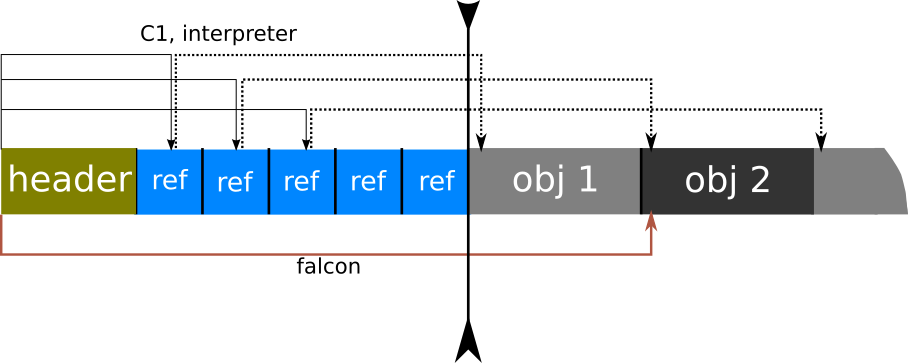
\includegraphics[width=0.95\linewidth]{image/flatarray.png}
\end{figure}
В реальности этот FlatArray представляет собой обычный Java массив класса Type[].class, у которого позади расположены элементы. Доступ к определенному элементу может быть осуществлен двумя способами: стандартным, через чтение и разыменование указателя, или путем вычисления адреса. 
JVM использует оба подхода. При интерпретации или исполнении С1 скомпилированного кода применяется первый подход, falcon - второй. 
Как упоминалось ранее, режим С1 и интерпретатор используют JNI методы для работы с FA. Однако при falcon компиляции JNI реализации подменяются специально подготовленными интринсиками. 
Свойство nullability достигается путем добавления поля 'isSentinel' во внутрь элемента. 
В конечном итоге такая раскладка FlatArray имеет ряд недостатков:
\begin{enumerate}
	\item Проверка nullability достаточно медленная. Особенно в случае not-existing, поскольку мы имеем большее число промахов кеша по сравнению с классическим Java массивом.
	\item Необходимо вычислять размер элемента массива для адресной арифметики, что дает значительные накладные расходы. Либо необходимо хранить размер элемента где-то внутри структуры данных, что и было применено в последствии.
	\item Нет поддержки сборки мусора, поскольку такой FlatArray неотличим от обычного Java массива объектов. 
	Необходимо корректно предоставлять метаинформацию о этом объекте. 
\end{enumerate}

\subsection{Представление с sentinel array}
В этом разделе представлена альтернативная версия раскладки полей FlatArray. В ней учтены недостатки предыдущего подхода.
\begin{figure}[h]
	\caption{Первая версия FlatArray}\label{first-fa}
	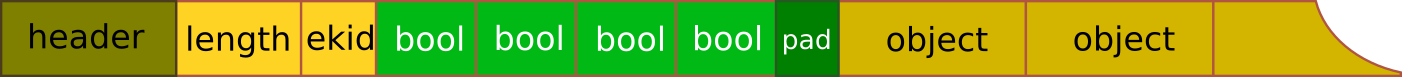
\includegraphics[width=0.95\linewidth]{image/flatarray-new.png}
\end{figure}
Этот массив состоит из следующих полей:
\begin{itemize}
	\item header[8 byte]; markWord этого объекта
	\item length [4 byte]; длина массива
	\item ekid [4 byte]; KID элемента массива
	\item sentinel array; массив элементов типа bool, который показывает, какие элементы внутри были явно инициализированы
	\item pad; поле для выравнивания 
	\item Последовательность элементов вместе с метаинформацией
\end{itemize}
Поля 'isSentinel' вынесены в одну компактную область памяти, что в итоге уменьшает число промахов кеша в режиме 'not-existing'.
Результаты тестирования производительности можно увидеть в таблицах \ref{sentinel-hashMap-perf1}, \ref{sentinel-hashMap-perf2} и \ref{sentinel-hashMap-perf3}:

\begin{table}[H]
	\centering
	\caption{Производительность HashMap only-existing.}\label{sentinel-hashMap-perf1}
	\textit{\begin{tabular}{|c|c|}
			\hline Benchmark  & Score, op/s \\
			\hline faMapLoop  & 5523 \\
			\hline mapLoop    & 5646 \\
			\hline 
	\end{tabular}}
\end{table}

\begin{table}[H]
	\centering
	\caption{Производительность HashMap fifty-fifty.}\label{sentinel-hashMap-perf2}
	\textit{\begin{tabular}{|c|c|}
			\hline Benchmark  & Score, op/s \\
			\hline faMapLoop  & 6122 \\
			\hline mapLoop    & 5833 \\
			\hline 
	\end{tabular}}
\end{table}

\begin{table}[H]
	\centering
	\caption{Производительность HashMap not-existing.}\label{sentinel-hashMap-perf3}
	\textit{\begin{tabular}{|c|c|}
			\hline Benchmark  & Score, op/s \\
			\hline faMapLoop  & 34216 \\
			\hline mapLoop    & 30371 \\
			\hline 
	\end{tabular}}
\end{table}
 
\subsection{Текущее представление}
Новое внутреннее представление FlatArray изображено на рисунке \ref{last-fa}
\begin{figure}[h]
	\caption{Текущее представление FlatArray}\label{last-fa}
	
\includegraphics[width=0.95\linewidth]{image/flat-array-without-sentinel.png}
\end{figure}
Этот массив имеет несколько полей:
\begin{itemize}
	\item markWord [8 byte]; 
	\item length [4 byte]; длина массива
	\item ekid [4 byte]; KID элемента массива
	\item Последовательность элементов вместе с метаинформацией:
		\begin{itemize}
			\item offset[4 byte]; Смещение от заголовка текущего элемента до заголовка FlatArray.
			\item bool[1 byte]; показывает, что данный элемент был инициализирован.
			\item pad; выравнивание.
			\item object; элемент массива.
		\end{itemize}
\end{itemize}
Результаты тестирования производительности можно увидеть в таблицах \ref{new-hashMap-perf1}, \ref{new-hashMap-perf2} и \ref{new-hashMap-perf3}: 
\begin{table}[H]
	\centering
	\caption{Производительность HashMap only-existing.}\label{new-hashMap-perf1}
	\textit{\begin{tabular}{|c|c|}
			\hline Benchmark  & Score, op/s \\
			\hline faMapLoop  & 6032 \\
			\hline mapLoop    & 5654 \\
			\hline 
	\end{tabular}}
\end{table}

\begin{table}[H]
	\centering
	\caption{Производительность HashMap fifty-fifty.}\label{new-hashMap-perf2}
	\textit{\begin{tabular}{|c|c|}
			\hline Benchmark  & Score, op/s \\
			\hline faMapLoop  & 5393 \\
			\hline mapLoop    & 5824 \\
			\hline 
	\end{tabular}}
\end{table}

\begin{table}[H]
	\centering
	\caption{Производительность HashMap not-existing.}\label{new-hashMap-perf3}
	\textit{\begin{tabular}{|c|c|}
			\hline Benchmark  & Score, op/s \\
			\hline faMapLoop  & 19401 \\
			\hline mapLoop    & 25757 \\
			\hline 
	\end{tabular}}
\end{table}
Как видно из таблиц, поиск существующего ключа в хеш-таблице, базирующейся на FlatArray, менее эффективно, чем в стандартной HashMap, однако в других случаях мы имеем хорошую производительность.
\textcolor{red}{оформление таблиц}
\begin{table}[H]
	\centering
	\caption{Производительность FlatArray only-existing.}\label{new-flatArray-perf1}
	\textit{\begin{tabular}{|c|c|}
			\hline Benchmark  & Score, op/s \\
			\hline faMapLoop  & 6032 \\
			\hline mapLoop    & 5654 \\
			\hline 
	\end{tabular}}
\end{table}

\begin{table}[H]
	\centering
	\caption{Производительность FlatArray not-existing.}\label{new-flatArray-perf3}
	\textit{\begin{tabular}{|c|c|}
			\hline Benchmark  & Score, op/s \\
			\hline faMapLoop  & 19401 \\
			\hline mapLoop    & 25757 \\
			\hline 
	\end{tabular}}
\end{table}

\clearpage